\begingroup
\newcommand{\GerlingSeconds}[2]{#1\makebox[.42em][c]{,\makebox[0pt][r]{\textsuperscript{s}}}#2}
\begin{center}
\textsc{Gauss} an \textsc{Gerling}.\quad Göttingen, 11.~August 1823.
\end{center}

\par\noindent\hspace*{\parindent}\mbox{.\ .\ .\ .\ .\ .\quad Ihre} Formulierung, \textls[120]{wenn} ich vom Brocken aus das Heliotroplicht anvisieren wolle und nicht das Häuschen vorzöge usw., scheint auf ein gewisses Missverständnis der Gründe hinzudeuten, aus denen ich ein zweites Mal auf den Brocken gehen könnte.
Die genaue Bestimmung der Richtung zum Inselsberg ist in der Tat ein Hauptzweck, und davon, das Haus anzuvisieren, kann bei dieser Entfernung und seiner geringen Höhe und unregelmäßigen Gestalt gar keine Rede sein.
Heliotroplicht vom Inselsberg zum Brocken ist also natürlich die Conditio sine qua non dafür, dass ich hingehe.
\par\noindent\hspace*{\parindent}Dieser eine Grund allein würde einen erneuten Besuch jedoch noch nicht rechtfertigen.
Meine Winkelmessungen von 1821 zu meinen
\par\clearpage
\noindent\null\hfill{\small\textbf{ZUR HANNOVERSCHEN TRIANGULATION.}}\hfill\makebox[0pt][r]{\fontsize{13}{16}\selectfont 383}\par\medskip
\noindent eigenen Hauptpunkten waren mit dem wandernden Heliotrop und bei ungünstigem Wetter zu dürftig und des ganzen Unternehmens nicht recht würdig ausgefallen. Daher wollte ich sie wiederholen, indem ich die Punkte gleichzeitig mit Heliotropen besetze, und später auch noch einmal zum Hohehagen und zum Hils zurückkehren.
\par\noindent\hspace*{\parindent}So gern ich Ihnen nun vom Brocken und vom Hohehagen zum Inselsberg Licht für Licht schicken will, kann ich Ihnen dafür doch keinen meiner Heliotrope überlassen. Denn wenn ich den Hohehagen, den Hils und vielleicht Lichtenberg mit einem einzigen wandernden Heliotrop besetzen müsste, käme ich nicht weiter als 1821.
\par\noindent\hspace*{\parindent}Mir scheinen mehrere Wege denkbar, um hier weiterzukommen:
\par\noindent\hspace*{\parindent}1) Wenn Sie und ich gleichzeitig zum Inselsberg bzw. zum Brocken kommen und uns gegenseitig Licht schicken und mein Gehilfe die Anweisung erhält, Ihnen von Zeit zu Zeit Licht vom Hohehagen zu schicken, und der Ihre mir vom Meisner, dann kann ich bei günstigem Wetter, wie es Anfang September häufig ist, in wenigen Tagen, vielleicht in dreien, auf dem Brocken fertig werden. Ich kann den Gehilfen mit dem Heliotrop dort lassen (er schickt Ihnen fortwährend Licht zum Inselsberg, ebenso wie der Gehilfe auf dem Hohehagen), zum Hohehagen eilen, Ihnen meine Ankunft signalisieren und dort in ein paar weiteren Tagen (bei günstigem Wetter) die Arbeiten abschließen, die den Inselsberg betreffen. Dann können Sie über Ihren Inselsberg-Heliotrop nach Belieben verfügen.
Vom Hohehagen erhalten Sie dann \textls[120]{ständig} Licht, solange ich dort bin, und wenn Sie es noch brauchen, hin und wieder, sobald ich auf dem Hils bin.
\par\noindent\hspace*{\parindent}Bei diesem Plan kommt es also ganz darauf an, ob Sie die Verbindung mit dem Brocken und den hannoverschen Dreiecken für wichtig genug halten, um die Besetzung des Knills und der Milseburg mit Heliotropen aufzuschieben, bis er ausgeführt ist.
\par\noindent\hspace*{\parindent}2) Obwohl mir der oben genannte Weg am liebsten wäre, weil so die Messungen am vollständigsten miteinander verbunden werden, könnten Sie den Inselsberg-Heliotrop \textls[120]{notfalls} schon früher abgeben, nämlich sobald ich den Brocken verlasse. Das lässt sich durch Signale mitteilen.
Für die Richtung Hohehagen–Inselsberg müsste ich mich dann mit dem begnügen, was ich 1821 mit \textsc{Enckes} Helio-
\par\clearpage
\noindent\makebox[0pt][l]{\fontsize{13}{16}\selectfont 384}\hfill{\small\textbf{BRIEFWECHSEL MIT GERLING.}}\hfill\null\par\medskip
\noindent trop erhalten habe.
Es versteht sich, dass Sie die Lage des neuen Steins und des Heliotropstandorts gegenüber dem \textls[120]{Haus} so genau wie möglich bestimmen müssten.
Ich wiederhole jedoch, dass es besser wäre, wenn ich auf dem Hohehagen den Winkel vom Inselsberg zum Brocken unmittelbar bestimmen könnte.
\par\noindent\hspace*{\parindent}3) Am besten wäre es wohl, wenn Sie sich gleich noch einen dritten Heliotrop anschafften.
Der Gewinn an Genauigkeit und Zeit, den Sie künftig dadurch hätten, würde den geringen Aufwand gewiss mehr als aufwiegen.
Das wäre jetzt umso leichter, als \textsc{Rumpf} gerade einen neuen Heliotrop fertig dastehen hat.
Er hat nämlich einen für \textsc{Schumacher} angefertigt (und bereits abgeschickt) und bei dieser Gelegenheit gleich zwei auf einmal hergestellt, weil es sich, wie er sagt, so leichter arbeiten lässt.
Der zweite ist also im Augenblick noch verfügbar, obwohl er gewiss auch sonst leicht Gelegenheit finden wird, ihn zu verkaufen.
(Bei mir sind bereits mehrere Anfragen aus dem Ausland eingegangen.)
Ich habe Herrn \textsc{Rumpf} gebeten, diesen Heliotrop ganz versandfertig zu machen und ihn niemand anderem zu geben, bevor Sie sich dazu erklärt haben.
Wenn Sie daran interessiert sind, ist es vielleicht am sichersten und schnellsten, ihn zum Meisner schicken oder ihn abholen zu lassen.
\par\noindent\hspace*{\parindent}4) Ich könnte auch etwas früher zum Brocken aufbrechen als Sie zum Inselsberg. Sie müssten dann versuchen, auf der Milseburg die Richtung zum Inselsberg vor allen anderen zu bestimmen, damit Ihr Gehilfe mir vom Inselsberg aus fortwährend Licht zum Brocken schickt, und zwar von dem noch zu vereinbarenden Tag an, an dem ich dort eintreffe.
So müssten Sie Ihren Heliotrop nach Ihrer eigenen Ankunft nur noch kürzere Zeit auf dem Inselsberg behalten.
\par\noindent\hspace*{\parindent}Sollte all dies aber mit Ihren Plänen unvereinbar sein, müsste ich auf die ganze Expedition verzichten, wenigstens für dieses Jahr (in diesem Fall bitte ich jedoch um möglichst baldige Nachricht, damit meine Gehilfen und ich uns danach richten können). Ich weiß auch nicht, ob ich mich im kommenden Jahr in demselben Maße danach richten könnte wie diesmal.
Diesmal biete ich nämlich an, Ihnen den Zeitpunkt des Beginns ganz zu überlassen.
Nennen Sie mir nur genau den \textls[120]{Tag}, von dem an Sie mir zuverlässig Licht vom Inselsberg zum Brocken schicken werden.
An diesem Tag bin ich bestimmt da, und in den Fällen 1,
\par\clearpage
\noindent\null\hfill{\small\textbf{ZUR HANNOVERSCHEN TRIANGULATION.}}\hfill\makebox[0pt][r]{\fontsize{13}{16}\selectfont 385}\par\medskip
\noindent 2, 3 schicke ich Ihnen auch sofort Heliotroplicht. Im Fall 4 tue ich das, sobald Ihr Licht das einfache Aufmerksamkeitszeichen nach den gewöhnlichen Uhrschlägen von \GerlingSeconds{0}{4} gibt, nämlich so:
\par\smallskip
{\centering
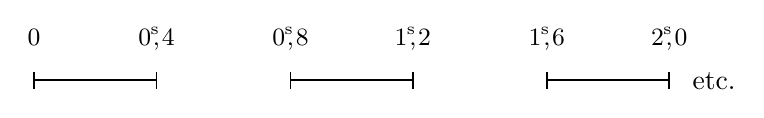
\begin{tikzpicture}[x=.0074cm,y=.0074cm,inner sep=0pt,outer sep=0pt,line width=.65pt]
\node[font=\small,anchor=base] at (0,60) {0};
\node[font=\small,anchor=base] at (210,60) {\GerlingSeconds{0}{4}};
\node[font=\small,anchor=base] at (440,60) {\GerlingSeconds{0}{8}};
\node[font=\small,anchor=base] at (650,60) {\GerlingSeconds{1}{2}};
\node[font=\small,anchor=base] at (880,60) {\GerlingSeconds{1}{6}};
\node[font=\small,anchor=base] at (1090,60) {\GerlingSeconds{2}{0}};
\draw (0,0)--(210,0) (0,-15)--(0,15) (210,-15)--(210,15);
\draw (440,0)--(650,0) (440,-15)--(440,15) (650,-15)--(650,15);
\draw (880,0)--(1090,0) (880,-15)--(880,15) (1090,-15)--(1090,15);
\node[anchor=base west] at (1130,-15) {etc.};
\end{tikzpicture}\par}
\par\noindent\hspace*{\parindent}Dabei merke ich jedoch an, dass der Spiegel stets ganz abgedeckt sein muss und dass die Abdeckungen eher etwas länger dauern müssen als die Öffnungen. Ich meine es so:
\par\smallskip
{\centering
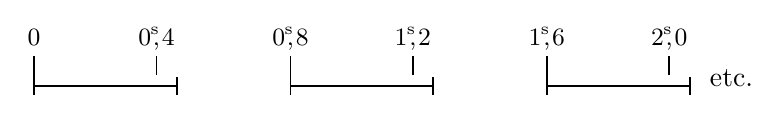
\begin{tikzpicture}[x=.0074cm,y=.0074cm,inner sep=0pt,outer sep=0pt,line width=.65pt]
\node[font=\small,anchor=base] at (0,70) {0};
\node[font=\small,anchor=base] at (210,70) {\GerlingSeconds{0}{4}};
\node[font=\small,anchor=base] at (440,70) {\GerlingSeconds{0}{8}};
\node[font=\small,anchor=base] at (650,70) {\GerlingSeconds{1}{2}};
\node[font=\small,anchor=base] at (880,70) {\GerlingSeconds{1}{6}};
\node[font=\small,anchor=base] at (1090,70) {\GerlingSeconds{2}{0}};
\draw (0,0)--(245,0) (0,-15)--(0,15) (245,-15)--(245,15);
\draw (440,0)--(685,0) (440,-15)--(440,15) (685,-15)--(685,15);
\draw (880,0)--(1125,0) (880,-15)--(880,15) (1125,-15)--(1125,15);
\draw (0,15)--(0,52) (210,20)--(210,52) (440,15)--(440,52) (650,20)--(650,52) (880,15)--(880,52) (1090,20)--(1090,52);
\node[anchor=base west] at (1160,-1) {etc.};
\end{tikzpicture}\par}
\par\noindent\hspace*{\parindent}Andere Zeichen gebe ich mit Zahlen, zum Beispiel die Zahl 3, nach folgendem Schema:
\par\noindent\hspace*{\parindent}\textls[120]{Ich} gebe eine unbestimmte Zahl von Aufmerksamkeitszeichen, bis\\
\hspace*{\parindent}\textls[120]{Sie} dieselben Zeichen erwidern, und zwar so lange, bis\\
\hspace*{\parindent}\textls[120]{ich} aufhöre, woraufhin Sie auch aufhören und \textls[120]{Acht} geben.
Inzwischen kann man etwa \(\frac{1}{4}\) Minute warten.
Dann gebe ich das Zeichen selbst, und zwar so:
\par\smallskip
{\centering
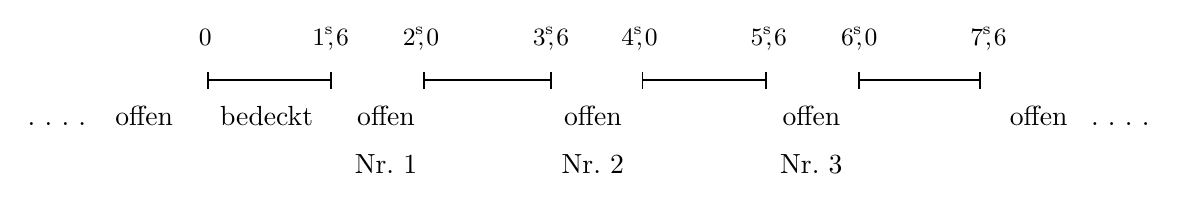
\begin{tikzpicture}[x=.0074cm,y=.0074cm,inner sep=0pt,outer sep=0pt,line width=.65pt]
\node[font=\small,anchor=base] at (360,60) {0};
\node[font=\small,anchor=base] at (575,60) {\GerlingSeconds{1}{6}};
\node[font=\small,anchor=base] at (730,60) {\GerlingSeconds{2}{0}};
\node[font=\small,anchor=base] at (953,60) {\GerlingSeconds{3}{6}};
\node[font=\small,anchor=base] at (1105,60) {\GerlingSeconds{4}{0}};
\node[font=\small,anchor=base] at (1327,60) {\GerlingSeconds{5}{6}};
\node[font=\small,anchor=base] at (1482,60) {\GerlingSeconds{6}{0}};
\node[font=\small,anchor=base] at (1704,60) {\GerlingSeconds{7}{6}};
\draw (365,0)--(575,0) (365,-15)--(365,15) (575,-15)--(575,15);
\draw (735,0)--(953,0) (735,-15)--(735,15) (953,-15)--(953,15);
\draw (1110,0)--(1322,0) (1110,-15)--(1110,15) (1322,-15)--(1322,15);
\draw (1482,0)--(1690,0) (1482,-15)--(1482,15) (1690,-15)--(1690,15);
\node[anchor=base west] at (55,-78) {\mbox{.\ .\ .\ .}};
\node[anchor=base] at (255,-78) {offen};
\node[anchor=base] at (465,-78) {bedeckt};
\node[anchor=base] at (670,-78) {offen};
\node[anchor=base] at (1025,-78) {offen};
\node[anchor=base] at (1400,-78) {offen};
\node[anchor=base] at (1790,-78) {offen};
\node[anchor=base west] at (1880,-78) {\mbox{.\ .\ .\ .}};
\node[anchor=base] at (670,-160) {Nr.~1};
\node[anchor=base] at (1025,-160) {Nr.~2};
\node[anchor=base] at (1400,-160) {Nr.~3};
\end{tikzpicture}\par}
\par\noindent\hspace*{\parindent}Setzt man die Zahl also \(=n\), so wechseln sich ab:
\par\smallskip
{\centering
\begin{tabular}{@{}r@{\quad}c@{\quad}l@{}}
 & \(n+1\) & Mal bedeckt, 4 Schläge lang,\\
mit & \(n\) & Mal offen, 1 Schlag lang (gleichsam \(n\) Blitze);
\end{tabular}\par}
\smallskip\noindent vorher und nachher, wie festgelegt, gewissermaßen unbegrenzt offen.
\par\noindent\hspace*{\parindent}Danach wiederholen Sie dasselbe Manöver in umgekehrter Richtung. Sofern jedoch keine \textls[120]{lange} Unterbrechung stattgefunden hat, warten Sie nicht auf meine Erwiderung Ihres Aufmerksamkeitszeichens. Nachdem Sie es etwa 10 bis 20-mal gegeben haben, machen Sie (offen) \(\frac{1}{4}\) Minute Pause und geben das Zeichen.
\par\noindent\hspace*{\parindent}Doppelte Zeichen, z.~B. \(3\,.\,3\), werden durch ein doppeltes Aufmerksamkeitszeichen angekündigt (\GerlingSeconds{0}{8} offen und \GerlingSeconds{0}{8} geschlossen). Nachdem die erste Zahl gegeben worden ist, bleibt der Spiegel etwa 5 bis \(10^{\mathrm{s}}\) lang offen, und dann wird die zweite Zahl gegeben, also so:
\par\smallskip\noindent\hspace*{.035\linewidth}{\scriptsize IX.}\hfill{\normalsize49}\hspace*{.14\linewidth}\par
\clearpage
\noindent\makebox[0pt][l]{\fontsize{13}{16}\selectfont 386}\hfill{\small\textbf{BRIEFWECHSEL MIT GERLING.}}\hfill\null\par\medskip
{\centering
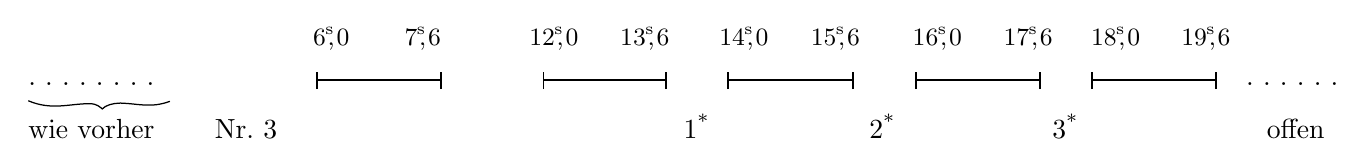
\begin{tikzpicture}[x=.0074cm,y=.0074cm,inner sep=0pt,outer sep=0pt,line width=.65pt]
\node[font=\small,anchor=base] at (540,60) {\GerlingSeconds{6}{0}};
\node[font=\small,anchor=base] at (697,60) {\GerlingSeconds{7}{6}};
\node[font=\small,anchor=base] at (922,60) {\GerlingSeconds{12}{0}};
\node[font=\small,anchor=base] at (1078,60) {\GerlingSeconds{13}{6}};
\node[font=\small,anchor=base] at (1248,60) {\GerlingSeconds{14}{0}};
\node[font=\small,anchor=base] at (1405,60) {\GerlingSeconds{15}{6}};
\node[font=\small,anchor=base] at (1580,60) {\GerlingSeconds{16}{0}};
\node[font=\small,anchor=base] at (1736,60) {\GerlingSeconds{17}{6}};
\node[font=\small,anchor=base] at (1886,60) {\GerlingSeconds{18}{0}};
\node[font=\small,anchor=base] at (2041,60) {\GerlingSeconds{19}{6}};
\draw (516,0)--(728,0) (516,-15)--(516,15) (728,-15)--(728,15);
\draw (904,0)--(1115,0) (904,-15)--(904,15) (1115,-15)--(1115,15);
\draw (1221,0)--(1435,0) (1221,-15)--(1221,15) (1435,-15)--(1435,15);
\draw (1544,0)--(1756,0) (1544,-15)--(1544,15) (1756,-15)--(1756,15);
\draw (1846,0)--(2058,0) (1846,-15)--(1846,15) (2058,-15)--(2058,15);
\node[anchor=base west] at (20,-8) {\mbox{.\ .\ .\ .\ .\ .\ .\ .}};
\draw[line width=.45pt] (20,-35) .. controls (60,-52) and (90,-40) .. (125,-40) .. controls (139,-40) and (144,-47) .. (147,-49) .. controls (152,-43) and (165,-39) .. (178,-39) .. controls (210,-40) and (230,-48) .. (263,-36);
\node[anchor=base west] at (20,-100) {wie vorher};
\node[anchor=base west] at (340,-100) {Nr.~3};
\node[anchor=base] at (1167,-100) {1\textsuperscript{*}};
\node[anchor=base] at (1486,-100) {2\textsuperscript{*}};
\node[anchor=base] at (1800,-100) {3\textsuperscript{*}};
\node[anchor=base west] at (2110,-8) {\mbox{.\ .\ .\ .\ .\ .}};
\node[anchor=base] at (2195,-100) {offen};
\end{tikzpicture}\par}
\par\noindent\hspace*{\parindent}Den Tag des Beginns überlasse ich, wie schon gesagt, Ihnen.
Ich muss nur so früh davon erfahren, dass ich nach Erhalt Ihres Briefes noch mindestens 4 bis 5 Tage Zeit habe, meinen Gehilfen in Hannover Anweisungen zu geben (denn jetzt ruhen die Arbeiten ganz), damit auch sie zur rechten Zeit vor Ort sind.
\par\noindent\hspace*{\parindent}Einen weiteren Umstand muss ich erwähnen.
Die Gehilfen auf dem Hohehagen und dem Meisner und gegebenenfalls, sobald ich auf dem Hohehagen bin, auch der Gehilfe auf dem Brocken müssen in 2 Richtungen Licht schicken, also abwechselnd.
\par\noindent\hspace*{\parindent}Sie werden die Zeit nun gleichmäßig aufteilen, einmal 1 Stunde oder 2 für den einen, dann für den anderen.
Es ist jedoch gut, wenn die Gehilfen jedes Mal, wenn sie wechseln wollen, dies etwa 5 Minuten vorher durch ein \(\frac{1}{2}\) Minute dauerndes Aufmerksamkeitszeichen ankündigen, damit [d]er [Beobachter] nicht Gefahr läuft, durch den plötzlichen Abbruch mitten in einer Beobachtungsreihe im Stich gelassen zu werden, sondern sie erst ordentlich abschließen kann.
Während ich auf dem Hohehagen bin, könnte Ihr Gehilfe mir wohl auch gelegentlich vom Meisner aus Licht schicken.
Inzwischen werde ich vermutlich auch den Stein selbst anvisieren können, sobald ich weiß, wo er steht, \textls[120]{wenn} er, worum ich bitte, \textls[120]{schwarz} gefärbt ist (mit Teer).
Doch darf der Gehilfe dann nicht unmittelbar am Stein stehen.
Weisen Sie ihn also an, sich ein Dutzend Schritte seitlich von der Richtung zum Hohehagen zu halten, und zwar vor allem \textls[120]{immer}, wenn die Sonne nicht scheint, und, wenn sie scheint, jedes Mal, sobald der Heliotrop eingestellt ist.
Vielleicht weisen Sie ihn auch an, schon vorher einmal Licht nach Göttingen zu schicken.
Vom 18.~dieses Monats an soll täglich zwischen 2 und \(2\frac{1}{2}\) Uhr Ausschau gehalten und der Empfang des Lichts durch eine Erwiderung angezeigt werden.
Ich fürchte aber, dass Ihr Gehilfe Mühe haben wird, die Richtung herauszufinden.
Wenn ich die Stelle wüsste, würde ich das Licht mit meinem eigenen herbeilocken.
Bis jetzt kann ich aber auf dem Gipfel mit dem Teleskop nichts sehen, was wie ein Stein aussieht.
Die höchste Stelle des Meisner ist von hier aus als ein (in senkrechter Richtung) schmaler Saum und als kahle Stelle oberhalb der Bäume sichtbar.
\par\clearpage
\noindent\null\hfill{\small\textbf{ZUR HANNOVERSCHEN TRIANGULATION.}}\hfill\makebox[0pt][r]{\fontsize{13}{16}\selectfont 387}\par\medskip
\par\noindent\hspace*{\parindent}Im Fall Nr.~4 würden Sie Ihre Ankunft auf dem Inselsberg dem Gehilfen auf dem Hohehagen dadurch mitteilen, dass Sie einmal Licht schicken.
Er liegt \(98^{0}\,28^{\prime}\) links von der Seeberger Sternwarte.
\par\noindent\hspace*{\parindent}Ich überlasse es Ihnen, ob Sie mir auch, wenn ich auf dem Hils bin, noch einmal Licht vom Meisner dorthin schicken lassen wollen.
Es würde jedenfalls zur vollständigen Verbindung beitragen.
Ich wollte das Licht schon selbst anfordern, da ich bis dahin den Standort genau genug kennen werde.
\par\noindent\hspace*{\parindent}Wenn es möglich ist, soll das Heliotroplicht von der Stelle aus, an der ich gerade selbst messe, genau in einer Linie mit dem Dreieckspunkt liegen. Geht das z.~B. auf dem Brocken nicht, wird die Abweichung natürlich genau gemessen.
\par\noindent\hspace*{\parindent}Am Hercules habe ich vom Hohehagen aus den Kopf anvisiert. Vom Brocken aus wurde der Hercules nur 4-mal mit dem Fadenkreuz eingestellt und dabei die ganze Station oder, genauer, die ganze pyramidenförmige Spitze des Oktogons anvisiert. --- Vom Hohehagen aus ist der Knill zwar unsichtbar. Ich vermute aber, dass Amöneburg sichtbar ist, vielleicht auch \mbox{Hohelohr.\quad.\ .\ .\ .\ .\ .}
\par
\endgroup
